\chapter{Introdução}\label{CAP:introducao}

Este documento descreve o desenvolvimento de um sistema para captação e análise de dados referentes à direção de um motorista.

A ideia básica é coletar dados de sensores já presentes em carros modernos através da porta OBD-II, que utiliza um padrão internacional de disponibilização de informações referentes a um carro\textsuperscript{[2]} e armazená-los em uma plataforma de dados, onde poderão ser posteriormente analisados.

\section{Motivação}

Qual o perfil de direção de um motorista? Como categorizar os condutores segundo um critério claro?

Buscando responder essas perguntas e, consequentemente, entender as características de pessoas ao volante, este trabalho propõe-se a criar uma infraestrutura de captura e análise de dados em automóveis de uso pessoal.

As informações recolhidas serão armazenadas em uma plataforma de nuvem, protegidas por algum nível de segurança, implementado neste mesmo projeto e, por fim, serão analisadas para gerarem conclusões interessantes sobre o modo de dirigir de cada participante do estudo.
	
Uma pesquisa preliminar sobre o assunto revelou que já existe uma patente para um produto parecido; ela foi registrada em 2013 e avalia o desempenho de um motorista a partir de dados pré-coletados de parâmetros relevantes à condução do carro \textsuperscript{[1]}.

Visão lateral do carro proposto na patente.[IMAGEM, REF 1]

[CITAR OS TRABALHOS QUE JÁ FAZEM ISSO QUE EU DISSE]

\section{Objetivo}

Este trabalho procura criar uma plataforma de disponibilização e captura de dados em um carro, coletando as informações \textit{in loco} e apresentando estatísticas relevantes derivadas do que foi coletado.

Para isso, fará uso da infraestrutura já presente em carros atuais, conforme pode ser visto na imagem a seguir, mas também pode complementá-la com mais equipamentos, caso seja necessário para o projeto.


\begin{figure}[hp]
    \centering
    
    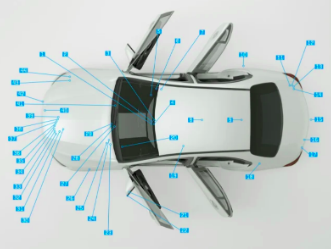
\includegraphics[]{figures/sensores_carro.png}
    
    \caption{Sensores estão presentes em um carro atual na ordem de dezenas\textsuperscript{[2]}}
\end{figure}

A coleta de dados será feita, a princípio, a partir de ensaios em carros reais feitos por uma quantidade seleta de pessoas, que pode ser expandida para resultados mais precisos na análise posterior.

Os dados coletados deverão ser passados para algum serviço de nuvem, usando conexão à \textit{internet}, caracterizando uma aplicação IoT.
	
Do lado da nuvem, será possível utilizar os dados de cada usuário de forma anônima, para diagnosticar o perfil do condutor e possivelmente gerar \textit{insights} sobre como a pessoa poderia melhorar.

 
\section{Justificativa}
% ROMEO e PIRES [GIT]
% Pq o trabalho é importante?
No ano de 2021, 11647 pessoas morreram em acidentes de trânsito no Brasil\textsuperscript{[6]}, além disso, no mundo inteiro morrem 1,35 milhão de pessoas em média, todos os anos\textsuperscript{[7]}, número comparável às mortes por Covid 19 até abril de 2022\textsuperscript{[8]}.

Levando-se em conta esses fatos, é simples entender a relevância deste projeto, pois ele define métricas importantes para classificação da conduta de motoristas, as quais podem ser usadas justamente para evitar acidentes e, portanto, preservar a vida humana.

É possível que no futuro os carros não sejam mais dirigidos por humanos ou que atuem por conta própria na maior parte das situações. Prevê-se, inclusive, que carros com nível de automação de pelos menos 4 comecem a se popularizar em 2025 \textsuperscript{[9]}.

Dessa forma, embora o fator humano venha a ser menos relevante para os acidentes do futuro, é preciso também haver métricas para classificar a condução dos veículos autônomos.

Este projeto tem, portanto, extrema relevância, pois é uma possível ferramenta para diminuir as mortes no trânsito, seja causada por pessoas ou por carros autônomos.

\section{Organização do trabalho}
% descrever sucintamente os capitulos e as demais parte dos trabalho


